\documentclass{foi}
\usepackage[utf8]{inputenc}
\usepackage{lipsum}

\vrstaRada{\projekt} % \diplomski \projekt \seminar \zavrsni
\title{Sustav za unos i analizu skupa riječi po rječniku - sustav zasnovan na
objektnom sustavu za upravljanje bazama podataka \texttt{ZODB}}

\author{Filip Novački}
\spolStudenta{\musko} % \zensko ili \musko
\mentor{Bogdan Okreša Đurić}
\spolMentora{\musko} % \zensko ili \musko
\godina{2020}
\mjesec{rujan}
%\date{2017}
%\status{redoviti}
\indeks{35918/07–R}
\smjer{Informacijski sustavi}
\titulaProfesora{dr. sc.}

\sazetak{Ovaj rad dokumentacija je projekta iz kolegija Teorija baza podataka.
Rad pokriva sve tehničke elemente projekta, pojedinosti baze, aplikacije te
cilja.}

\kljucneRijeci{ZODB, baza podataka, objektna baza podataka, flask, python,
server, neurolingvistika, riječi}

\begin{document}

\maketitle
\tableofcontents

\chapter{Uvod}

Ovo je projektna dokumentacija projekta za kolegij Teorija baza podataka na
diplomskom studiju na Fakultetu organizacije i informatike Sveučilišta u
Zagrebu. Cilj projekta je demonstrirati koncepte baza podataka koji nisu
uobičajeni kao što su relacijske baze podataka ili se radi o naprednijim
funkcionalnostima relacijskih baza.

Glavna tema ovog projekta je \texttt{ZODB} baza podataka te aplikacija koja se
njom koristi kao glavnim izvorom podataka.

\chapter{Opis projekta}

\section{Opis aplikacijske domene}

Domena ovog projekta stvaranje je rječnika i analiza riječi. Analizu riječi
omogućuju biblioteke za neurolingvističko programiranje koje imaju poprilično
širok fond raznih funkcionalnosti kojima se riječi mogu analizirati.

Glavna funkcionalnost za korisnika je vrlo jednostavna, a vrlo je intenzivna sa
strane poslužitelja koji radi niz koraka kako bi ju ostvario:
\begin{itemize}
	\item unos teksta
	\item čišćenje teksta i odvajanje riječi
	\item analiza riječi
	\item unos u bazu podataka.
\end{itemize}

Unos teksta zapravo nije predviđen kao proces gdje korisnik \textit{unosi}
tekst, već kao proces gdje korisnik lijepi veću količinu teksta (članci, objave
itd.) te se daje aplikaciji na analizu. Taj tekst ne mora biti ni na koji način
prilagođen -- aplikacija je sposobna u potpunosti izbaciti viškove kao što su
točke, zarezi i drugi znakovi, riječi bez značenja, brojeve (znamenke), kratke
riječi koje ne nose značenje nego su isključivo pomoćne naravi (en.
\textit{stopwords}) itd.

Analiza riječi je proces u kojem se unesenim riječima pripasuje značenje,
izgovor, vrsta riječi i ostale informacije te se pripremaju za spremanje u
bazu. Unatoč tome što je ovo vrlo jednostavno opisati u prirodnom jeziku,
upravo ovaj korak poslužitelju traje najduže.

Unos u bazu podataka korak je gdje se pripremljene informacije zapisuju u bazu.
Kod unosa obraća se pozornost na rječnik u kojeg se nešto dodaje i na već
postojeće riječi kako ne bi došlo do zapisivanja duplikata.

%11
-----------

Osim osnovne funkcionalnosti, aplikacija generira engleski rječnik iz rječnika
koji se nalazi u bazi podataka.

\section{Teorijska podloga baze podataka}

\texttt{ZODB} je objektno orijentiran sustav za upravljanje bazama podataka
pisan u Pythonu. To znači da se u bazu pohranjuju objekti kojima se kasnije
pristupa. Kad govorimo o spremanju objekata u Pythonu moramo se prisjetiti
biblioteke \texttt{pickle} koja služi za serijalizaciju objekata iz Pythona u
datoteke. Kombinacija ta dva pristupa omogućuju spremanje podataka u
hijerarhiju koja je nalik Pythonovim objektima, a spremljena je na disku
računala.

Takav pristup omogućuje pristupanje svim objektima, odnosno cijeloj bazi bez
uporabe prilagođenog jezika kao što je \texttt{SQL} te se pristup podatcima
može jako dobro integrirati u ostatak koda.

Objekti koji se spremaju u objektnu bazu moraju naslijediti klasu
\texttt{Persistent} iz biblioteke \texttt{persistent} ili se moraju koristiti
\textit{non-mutable} objekti kao što su n-torke (\textit{tuples}), stringovi i
drugi jednostavni tipovi podataka. Od tipova podataka ugrađenih u Python
promjenjivi (\textit{mutable}) su liste (\texttt{list}), rječnici
(\texttt{dict}) i skupovi (\texttt{set}).

Za tipove podataka koji jesu promjenjivi napravljeni su posebni tipovi koji se
ponašaju slično Pythonovim pretpostavljenim tipovima podataka, a prilagođeni su
za korištenje u \texttt{ZEO} serverima, a tako su i primjenjivi u \texttt{ZODB}
bazama podataka.

Kod stvaranja vlastitih klasa koje nasljeđuju klasu \texttt{Persistent}
potrebno je i promijeniti varijable koje označavaju jesu li se dogodile
promjene u toj klasi, odnosno varijablu \texttt{\_p\_changed} je potrebno
postaviti na \texttt{True}. Tako \texttt{ZODB} \textit{zna} da se promjena
dogodila i da je potrebno ponovno pohraniti taj objekt u bazu.

\section{Model baze podataka}

Na slici \ref{uml_db} prikazan je model baze podataka. Kod korištenja objektne
baze podataka jednostavnije je koristiti UML dijagram umjesto ERA modela unatoč
tome što izgledaju slično za danu bazu. Ovakav model ostavlja mjesto i za
popisivanje metoda koje se nalaze u pojedinoj klasi, no i to se izbjegava u
ovom slučaju s obzirom na to da poslovnu logiku nije potrebno spremati u bazu
podataka.

\begin{figure}[!h]
\centering
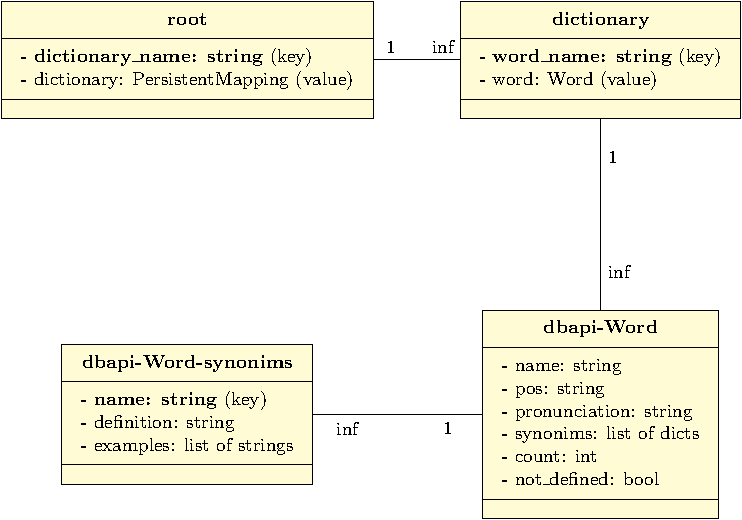
\includegraphics[scale=1]{uml_db.pdf}
\caption{Model baze podataka prikazan pomoću UML diagrama. Kvadrati su
	klase, masno otisnuti su ključevi, a tipovi podataka su iza dvotočja.
	Veze između klasa slovima su označene na vezama.}
\label{uml_db}
\end{figure}

Za ovu domenu objektna baza je izrazito učinkovita jer su klase nekoliko puta
ugniježđene jedna u drugu, a u relacijskoj bazi podataka bi to moglo biti
neučinkovito jer se za traženje pojedine vrijednosti moraju proći svi ostali
objekti, odnosno zapisi, kojih može biti izrazito mnogo. Zbog pristupa koji je
zasnovan na rječnicima, taj problem je spriječen jer se rječnici u Pythonu
indeksiraju i pristup im je brz, a svaki objekt koji pripada rječniku ima
direktnu vezu spremljenu do njega.

\section{Implementacija baze podataka}

Kao kratki uvod u implementaciju na slici \ref{project_diagram} prikazana je
karta projekta.

\begin{figure}[!h]
	\centering
	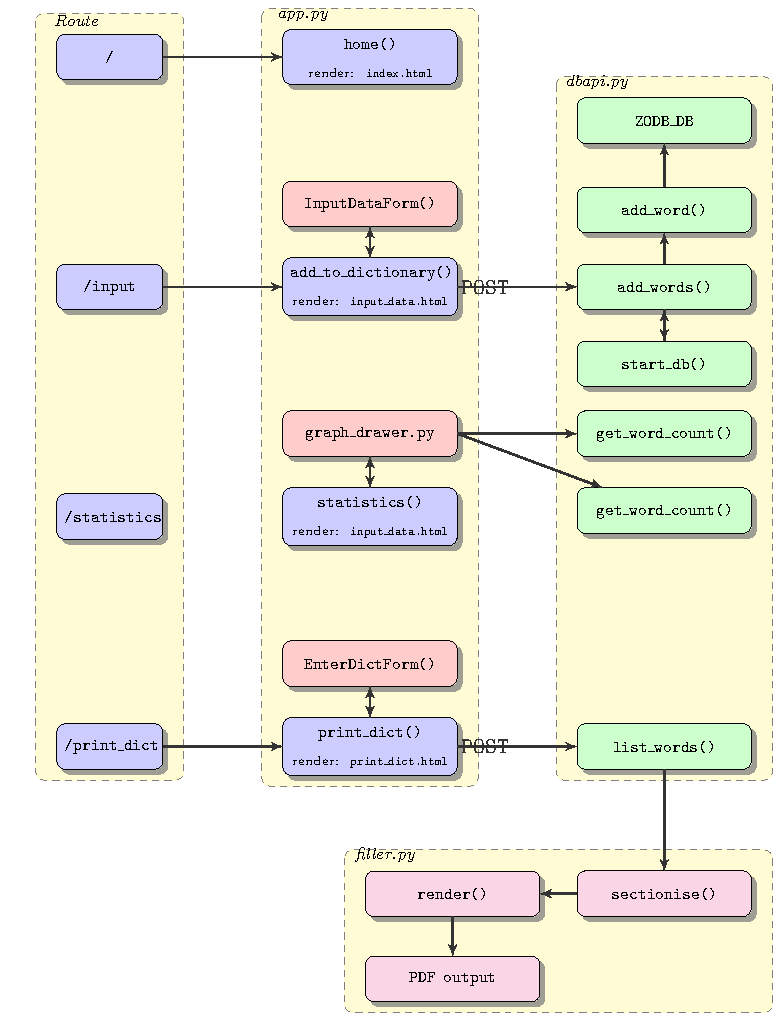
\includegraphics{project_diagram.pdf}
	\caption{Karta projekta s prikazanim značajnim točkama u kodu}
	\label{project_diagram}
\end{figure}

Projekt je napravljen od ovih glavnih elemenata:
\begin{itemize}
	\item \texttt{Flask} server
	\item ZODB baza podataka
\end{itemize}

\texttt{Flask} server poslužuje cijelu aplikaciju i prikazuje ju sučelju koje
je prilagođeno za web preglednike. \textit{Frontend} je izrazito jednostavan -
ne koristi se \texttt{JavaScript}, a \texttt{CSS} koji se koristi je
\texttt{Bulma}, \textit{open source} projekt koji pristojno i jednostavno
izgleda, a značajno poboljšava korisničko iskustvo nad pretpostavljenim
izgledom \texttt{HTML} datoteka.

Sama aplikacija vrlo je jednostavna i nalazi se u datoteci \texttt{app.py}. Na
slici \ref{project_diagram} razložena je podjela aplikacije tako da se vide putanje s koje
se aktiviraju određene funkcije. Tako na putanji \texttt{/} aktivira se funkcija
\texttt{home()} te se renderira \texttt{index.html}. Za renderiranje
\texttt{HTML}-a koristi se \texttt{Jinja}, biblioteka koja je integrirana u
\texttt{Flask}.

Osim za renderiranje \texttt{HTML}-a \texttt{Jinja} se koristi i za
renderiranje \LaTeX\ dokumenta - predložak za rječnik puni se podatcima iz baze
te se renderira.

Na sličan način kao što je opisano radi i ostatak aplikacije stoga on neće biti
u detalje opisan ovdje.

\subsection{Korištene tehnologije}

Kao što je već napomenuto, glavne okosnice projekta su \texttt{Flask} i
\texttt{ZODB} koji pokreću cijeli sustav. Osim tih tehnologija korišteni su i:
\begin{itemize}
	\item[\texttt{Jinja}] -- renderiranje \texttt{HTML}-a i \LaTeX-a
	\item[\texttt{persistent}] -- tipovi podataka za rad s bazom podataka
	\item[\texttt{nltk}] -- većina obrade riječi i dobavljanje njihovog
		značenja
	\item[\texttt{textblob}] -- također za obradu riječi, ali na višoj
		razini od \texttt{nltk}-a. \texttt{textblob} je implementiran
		funkcijama \texttt{nltk}-a
	\item[\texttt{os}] -- Pythonova biblioteka za rad s naredbama
		operacijskog sustava, korišteno za pokretanje naredbi u ljusci
		te za provjeravanje postojećih datoteka u sustavu
	\item[\texttt{wtforms}] -- biblioteka za kreiranje formi, integrirano s
		\texttt{Flaskom} i \texttt{Jinjom}
	\item[\texttt{matplotlib}] -- Pythonova biblioteka za crtanje grafova
	\item[\LaTeX] -- služi za renderiranje PDF datoteke iz teksta
	\item[ostalo] -- nekoliko Pythonovih biblioteka za rad s operacijskim
		sustavom, uglavnom korišteno za uredan rad s \LaTeX-om
\end{itemize}

\subsection{Problemi u implementaciji}

S obzirom na to da se ovaj projekt bavi bazama podataka, manje se pozornosti
stavljalo na korisničko iskustvo. S tim u vidu jedan problem ostaje neriješen
-- rad stranice za vrijeme intenzivnog rada s bazom.

U slučaju kad se javi neki malo intenzivniji poduhvat za bazu dogodi se da se
stranica ne učita dok se sva obrada ne dovrši, odnosno procesuiranje se odvija
sinkrono. U projektu se taj problem događa u najmanje dva slučaja:
\begin{itemize}
	\item unos riječi
	\item dohvaćanje riječi iz baze
\end{itemize}

Problem kod unosa riječi je taj što analiza riječi dugo traje -- pregledava se
baza engleskih riječi koja ima preko 130 kilozapisa, a iz te baze se izvlače
izgovori, sinonimi, vrste riječi i objašnjenja sinonima. Trenutno rješenje radi
tako da se slijedno analiziraju i zapisuju podatci, a rješenje problema bi bilo
da se poslužitelju predaje lista riječi, a da on u pozadini obrađuje dane
riječi, a da aplikacija dalje normalno radi. Osim asinkronog pristupa, moguće
je i pokrenuti drugi poslužitelj koji će raditi isključivo obradu podataka te na taj
način rasteretiti poslužitelj na kojem je aplikacija. To je također asinkroni
pristup, ali se pristup razlikuje u osnovnom principu koji ga pokreće.

Također je moguće i ostaviti učitavanje kako jest te pomoću
\texttt{JavaScripta} i \texttt{AJAX} tehnologije napraviti učitavanje stranice,
no to je ipak tema za neki drugi projekt.

Kod dohvaćanja liste riječi postoji problem ukoliko se ponovno pozove funkcija
za prikaz rječnika, a baza podataka se u međuvremenu nije zaključala. Ukoliko
se to dogodi, aplikacija pokušava otključati već otključanu bazu i aplikacija
se ruši. Iz tog se razloga korisnika moli za oprez.

\subsection{Problematika implementacije baze podataka}

Baza podataka implementirana je u Pythonu koristeći funkcije baze. Unatoč tome
što su \texttt{ZODB} baze podataka predviđene za neupadljivu integraciju u
ostatak Python koda, korisno je bilo odvojiti funkcije baze podataka od
serverske logike te od poslovne logike.

Osim toga, \texttt{ZODB} baza jako je osjetljiva na istovremeni pristup
podatcima te na pristupanje objektima kad je baza zaključana. Stoga je idealno
bazu držati što kraće otključanom, pristupiti podatcima i neposredno nakon toga
zaključati ju.

Problem na koji se može naići u pisanju aplikacije za bazu podataka je u
slučaju da korisnik želi neku klasu koja je pospremljena u bazi koristiti za
obradu. Jedna opcija je napraviti obradu za vrijeme dok je baza otključana, a
druga je da se napravi novi objekt u koji će se ti podatci zapisati. To su
jedine dvije opcije jer nakon što se baza zaključa nije moguće pristupiti
objektu koji je u bazi unatoč tome što u programu postoji referenca na taj
objekt.

\chapter{Prikaz rada i korištenje}

\section{Unos riječi}

Ova je aplikacija izrazito jednostavna za korištenje jer korisnik ima jako malo
toga što može učiniti u cijelom procesu.

\begin{figure}[!h]
	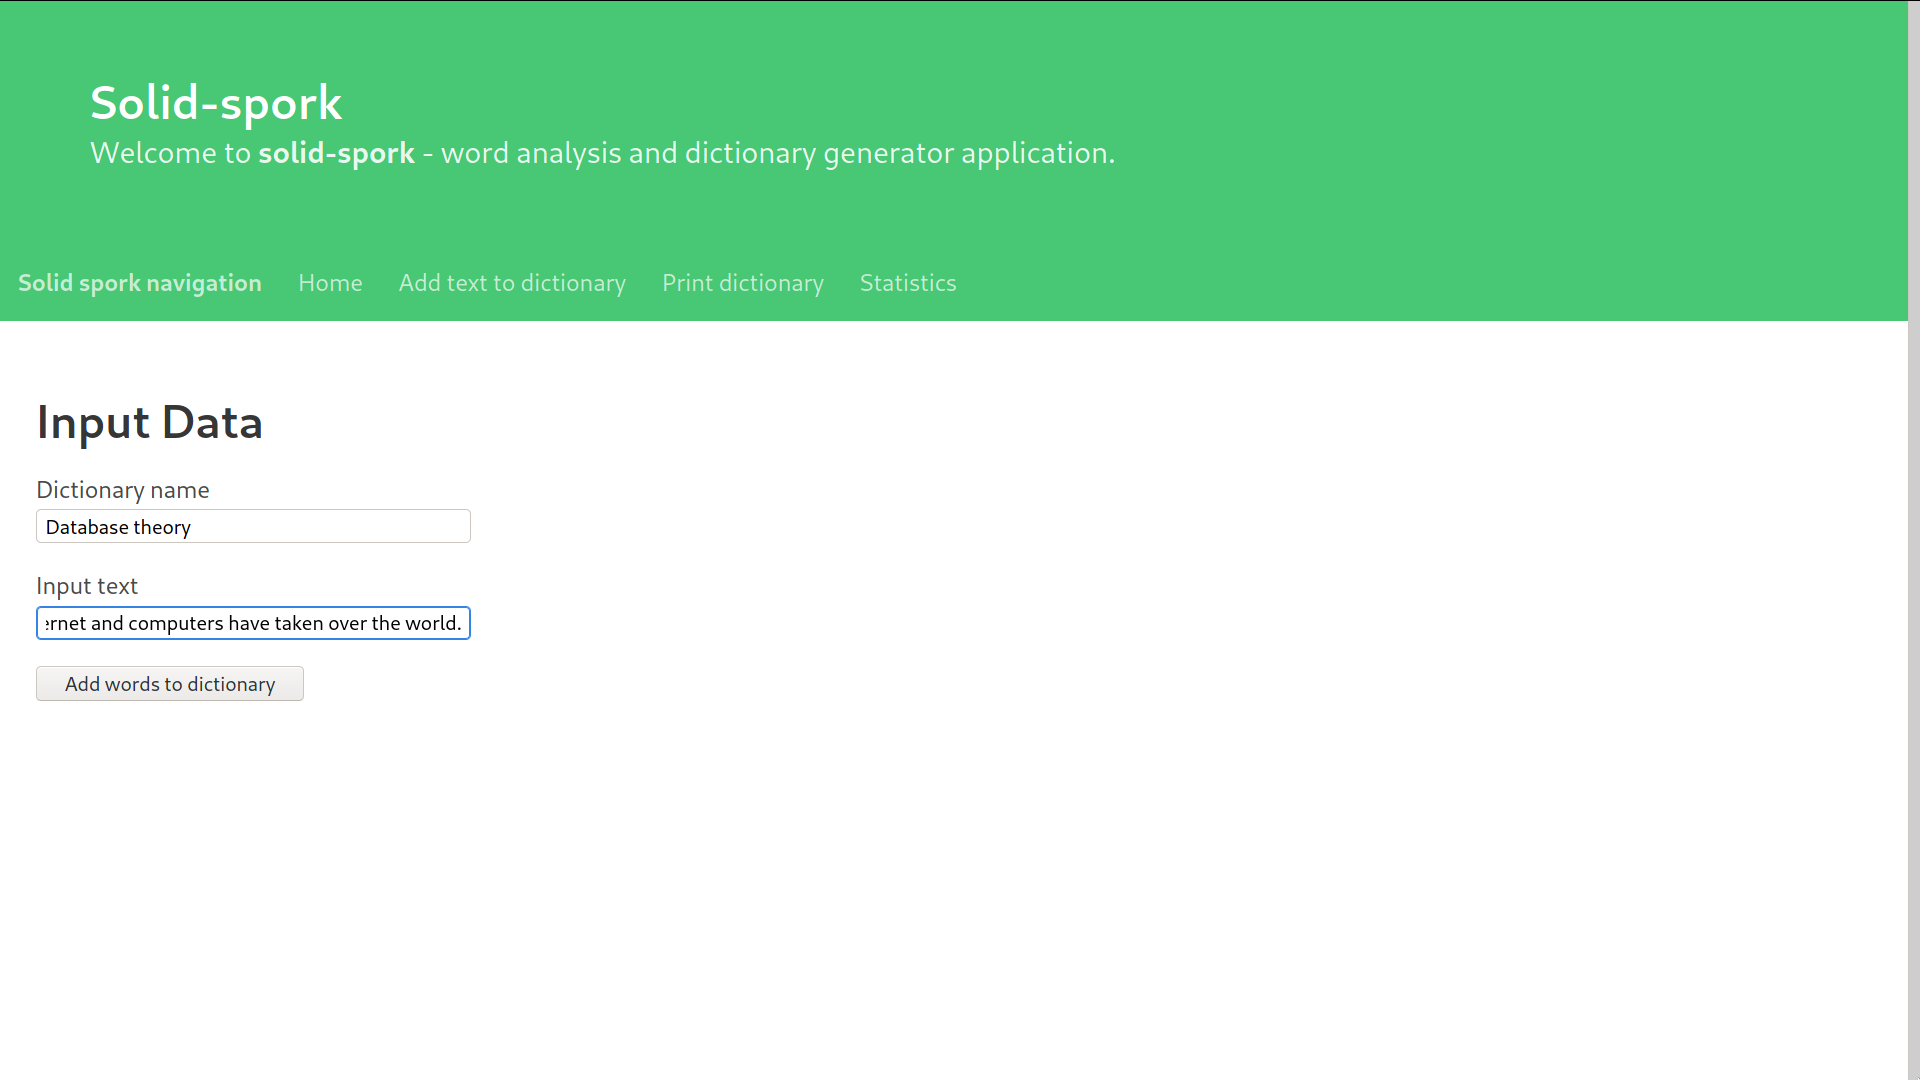
\includegraphics[width=\textwidth]{slike/solid-spork-input.png}
	\caption{Prikaz unosa teksta u bazu}
	\label{ht_unos}
\end{figure}

Na slici \ref{ht_unos} prikazan je prizor kako se riječi mogu unositi. Količina
podataka koja se može unijeti u polje ograničen je isključivo diskovnim
prostorom koji se na iole suvremenim računalima neće tako lako dostići.

Ovdje se preporuča unos velike količine teksta kao što su članci, blog objave
itd. Kod unosa većih količina teksta korisnik se moli za strpljenje jer je
potrebno oko pola sekunde po riječi zbog intenzivne obrade koja slijedi
nakon unosa.

\section{Ispis rječnika}

Ispis rječnika korak je koji je glavna motivacija koja stoji iza projekta (v.
slika \ref{ht_print}). Sve prikupljene riječi u nekom rječniku završavaju u
\LaTeX\ dokumentu i kompajliraju se po odabiru rječnika.

\begin{figure}[!h]
	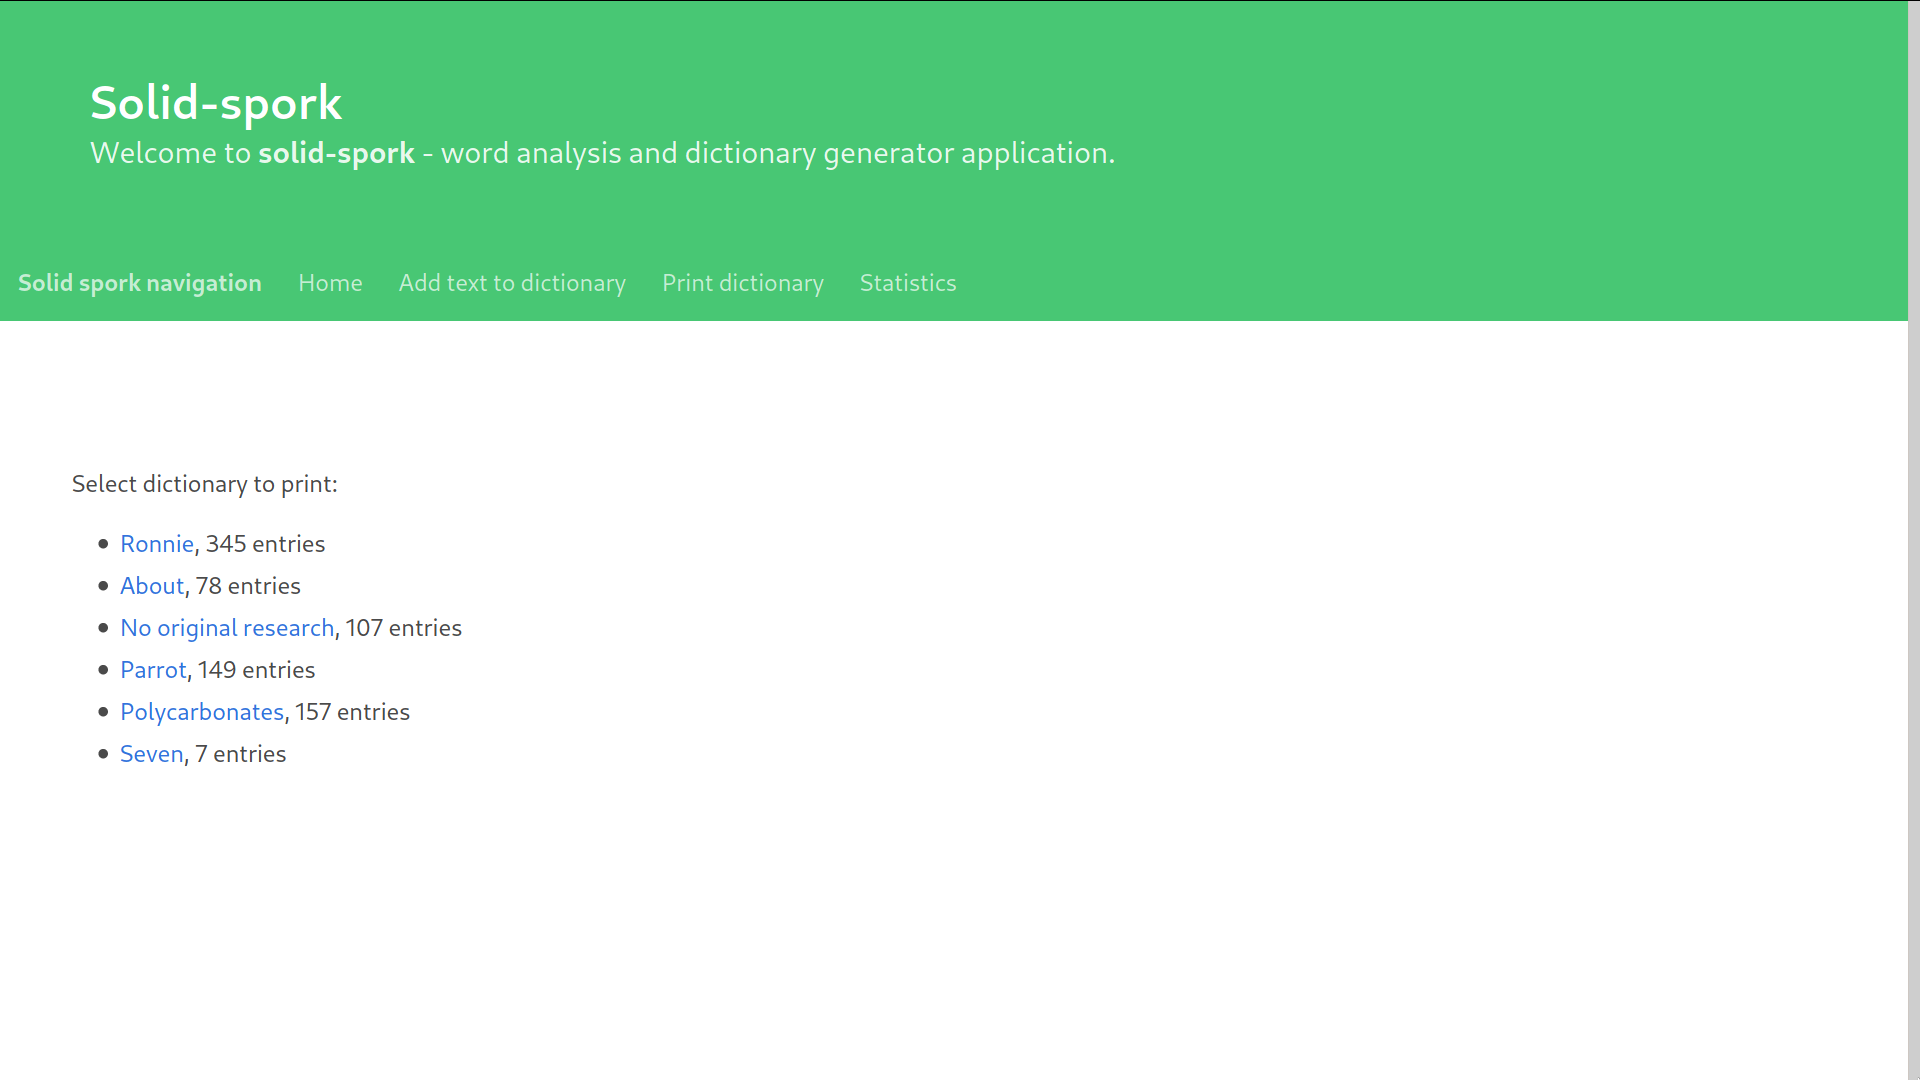
\includegraphics[width=\textwidth]{slike/solid-spork-print.png}
	\caption{Prikaz ispisa rječnika}
	\label{ht_print}
\end{figure}

Jednostavnim pritiskom na jedan od rječnika generira se PDF te se korisniku
daje na preuzimanje.

\section{Prikaz statistika}

Prikaz statistika je funkcionalnost koja ne zahtijeva nikakvu korisničku
intervenciju, već je isključivo informativne prirode. Na slici \ref{ht_stats}
prikazan je primjer jednog grafa, a ostali se pojavljuju ispod njega.

\begin{figure}[!h]
	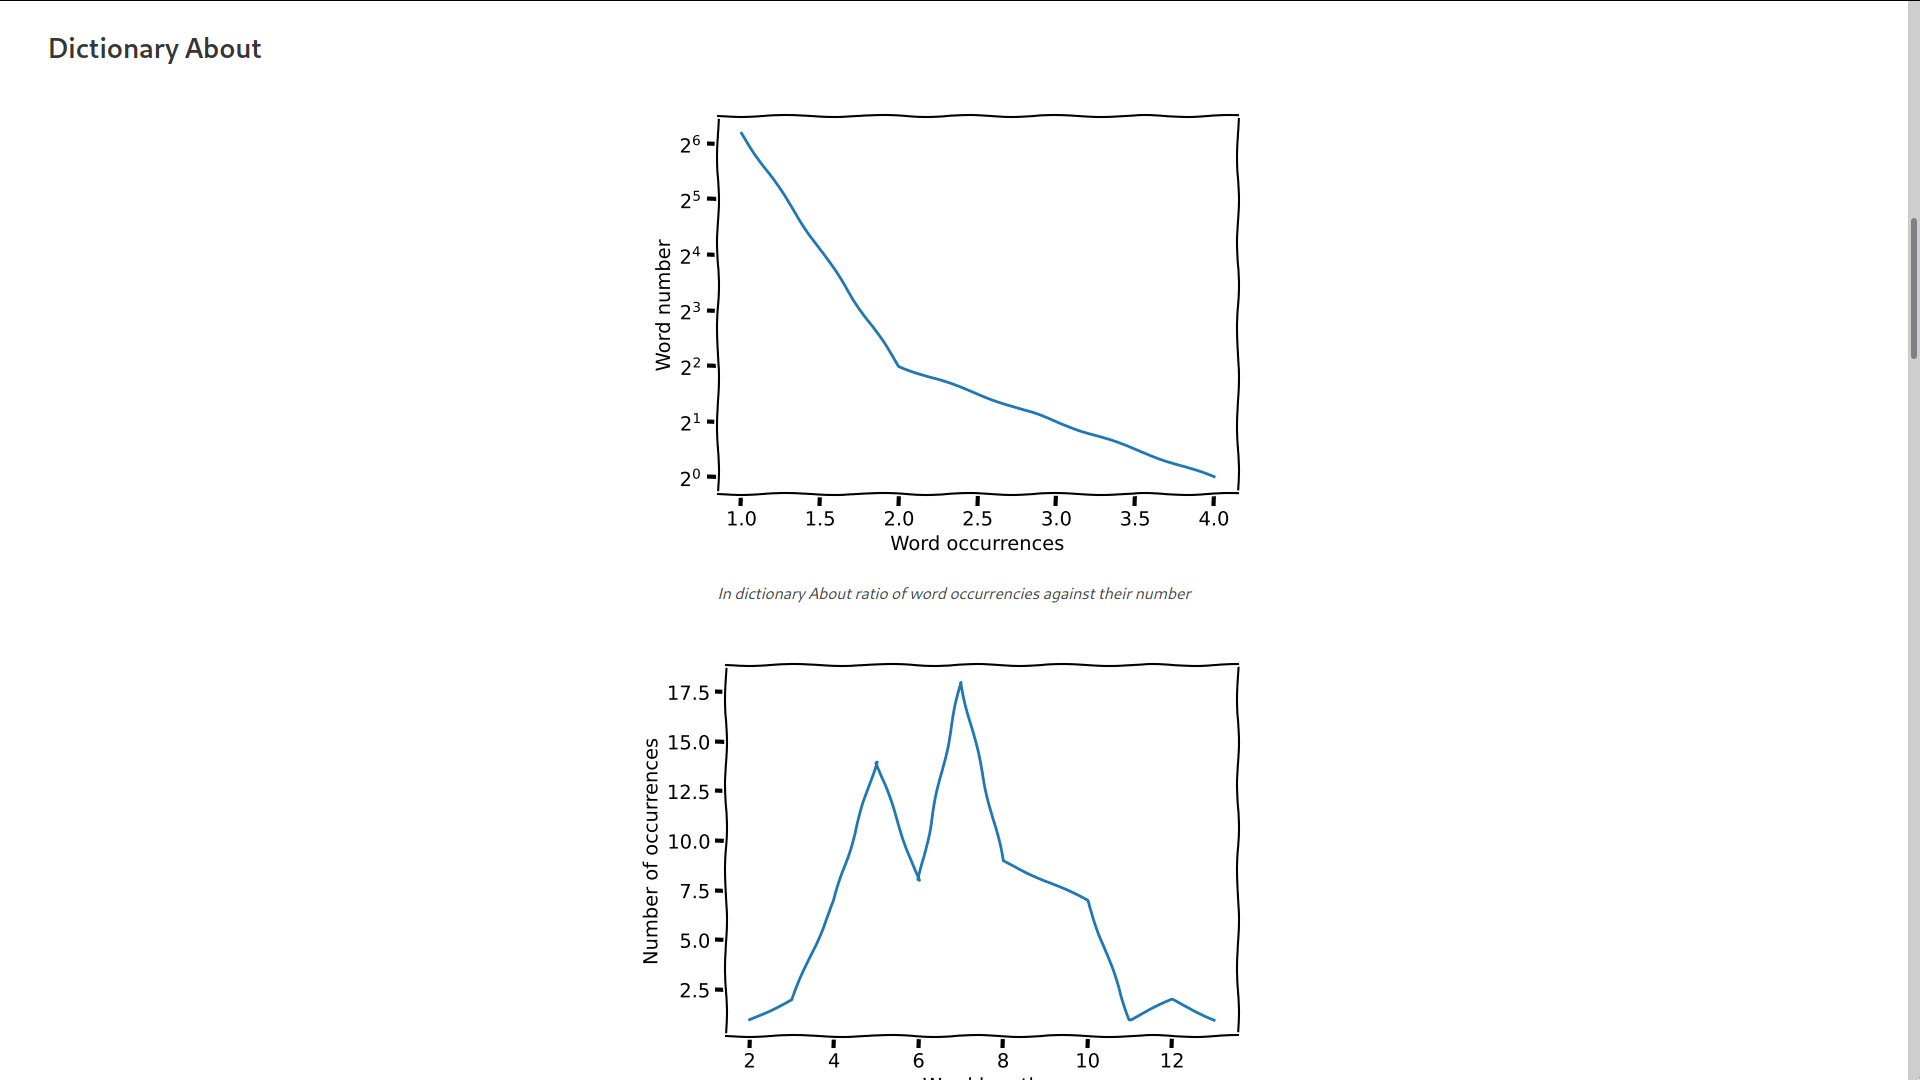
\includegraphics[width=\textwidth]{slike/solid-spork-stats.png}
	\caption{Prikaz ispisa rječnika}
	\label{ht_stats}
\end{figure}

Na grafovima su vizualno prikazana dva fenomena jezika - zastupljenost riječi
te duljina riječi. Prvi graf u nizu prikazuje koliko riječi ima određenu
frekvenciju. U svim je jezicima pravilo da svega nekoliko riječi se pojavljuje
najviše puta, a najviše riječi se pojavljuje jako malo puta. Također, jezik je
pun hapakslegomenona - riječi koje se pojavljuju samo jednom u nekom opusu.

Drugi graf pokazuje kojih je riječi prema duljini najviše. Odoka se primjećuje
nešto nalik na Poissonovu razdiobu, što bi se vjerojatno i moglo provjeriti
nekim sofisticiranijim metodama od odokativne metode.

\pagestyle{plain}

%\printbibliography[title=Popis literature]
\addcontentsline{toc}{chapter}{Popis literature}

\listoffigures
\addcontentsline{toc}{chapter}{Popis slika}

\listoftables
\addcontentsline{toc}{chapter}{Popis popis tablica}

\appendix
\renewcommand{\thechapter}{\arabic{chapter}}

\chapter{Prilog 1}

\chapter{Prilog 2}

\end{document}
